\documentclass[fontset=windows,12pt]{article}

\usepackage[UTF8]{ctex}
\usepackage[a4paper]{geometry}
\usepackage{amsmath}
\usepackage{fancyhdr}
\usepackage{amsthm}
\usepackage{amssymb}
\usepackage{xcolor}
\usepackage{listings}
\usepackage{graphicx}
\usepackage{circuitikz}
\ctikzset{logic ports=ieee}     %所有逻辑门使用IEEE标准
\usetikzlibrary{calc}           %使用TikZ中的计算功能
\setlength{\headheight}{14.49998pt}

\newtheorem{question}{\hskip 1.7mm \bf}
\renewenvironment{proof}{{\noindent\hskip 2em \bf ֤证明 \quad}}{\hfill$\qed$\par}
\newenvironment{solution}{{\noindent\hskip 2.4em \bf 解 \quad}}

\geometry{left=2.0cm,right=2.0cm,top=2.5cm,bottom=2.5cm}
\begin{document}

\definecolor{CPPLight}  {HTML} {686868}
\definecolor{CPPSteel}  {HTML} {888888}
\definecolor{CPPDark}   {HTML} {262626}
\definecolor{CPPBlue}   {HTML} {4172A3}
\definecolor{CPPGreen}  {HTML} {487818}
\definecolor{CPPBrown}  {HTML} {A07040}
\definecolor{CPPRed}    {HTML} {AD4D3A}
\definecolor{CPPViolet} {HTML} {7040A0}
\definecolor{CPPGray}  {HTML} {B8B8B8}
\lstset{
    columns=fixed,       
    numbers=left,                                        % 在左侧显示行号
    frame=none,                                          % 不显示背景边框
    backgroundcolor=\color[RGB]{245,245,244},            % 设定背景颜色
    keywordstyle=\color[RGB]{40,40,255},                 % 设定关键字颜色
    numberstyle=\footnotesize\color{darkgray},           % 设定行号格式
    commentstyle=\it\color[RGB]{0,96,96},                % 设置代码注释的格式
    stringstyle=\rmfamily\slshape\color[RGB]{128,0,0},   % 设置字符串格式
    showstringspaces=false,                              % 不显示字符串中的空格
    language=c++,                                        % 设置语言
    morekeywords={alignas,continute,friend,register,true,alignof,decltype,goto,
    reinterpret_cast,try,asm,defult,if,return,typedef,auto,delete,inline,short,
    typeid,bool,do,int,signed,typename,break,double,long,sizeof,union,case,
    dynamic_cast,mutable,static,unsigned,catch,else,namespace,static_assert,using,
    char,enum,new,static_cast,virtual,char16_t,char32_t,explict,noexcept,struct,
    void,export,nullptr,switch,volatile,class,extern,operator,template,wchar_t,
    const,false,private,this,while,constexpr,float,protected,thread_local,
    const_cast,for,public,throw,std},
    emph={map,set,multimap,multiset,unordered_map,unordered_set,
    unordered_multiset,unordered_multimap,vector,string,list,deque,
    array,stack,forwared_list,iostream,memory,shared_ptr,unique_ptr,
    random,bitset,ostream,istream,cout,cin,endl,move,default_random_engine,
    uniform_int_distribution,iterator,algorithm,functional,bing,numeric,},
    emphstyle=\color{CPPViolet}, 
}
\newenvironment{correction}{\par\noindent{\color{blue}{\bf{更正\\}}}\quad\color{blue}}{\par}
\pagestyle{fancy}
\lhead{中国科学院大学}
\chead{\bf{2024-25秋数字电路课程}}
\rhead{\emph{2023K8009929044 薛翼舟}}


\begin{center}
\huge{\bf{2024.10.20作业}}
\end{center}

\section{教材4-35 实现4位超前加法器}
    {\setmainfont{Courier New Bold}                          % 设置代码字体                   
    \begin{lstlisting}
module HC283(
    input [3:0]A,
    input [3:0]B,
    input Cin,
    output [3:0]S,
    output Cout
    );
    wire [3:0]C;
    wire [3:0]P;
    wire [3:0]G;
    integer i;
    
    assign C[0] = Cin;
    
    assign P[0] = A[0] ^ B[0];
    assign P[1] = A[1] ^ B[1];
    assign P[2] = A[2] ^ B[2];
    assign P[3] = A[3] ^ B[3];
    
    assign G[0] = A[0] & B[0];
    assign G[1] = A[1] & B[1];
    assign G[2] = A[2] & B[2];
    assign G[3] = A[3] & B[3];
    
    assign S[0] = P[0] ^ C[0];
    assign S[1] = P[1] ^ C[1]; 
    assign S[2] = P[2] ^ C[2]; 
    assign S[3] = P[3] ^ C[3]; 
    
    assign C[0] = Cin;
    assign C[1] = G[0] || (P[0] & C[0]);
    assign C[2] = G[1] || (P[1] & (G[0] || (P[0] & C[0])));
    assign C[3] = G[2] || 
    (P[2] & (G[1] || (P[1] & (G[0] || (P[0] & C[0])))));
    assign Cout = G[3] || //装不下了, 只能换行了
    (P[3] & (G[2] || (P[2] & (G[1] || (P[1] & (G[0] || (P[0] & C[0])))))));
endmodule
    \end{lstlisting}}

\section{教材4-36根据下面的语言描述, 画出对应的逻辑电路图}
{\setmainfont{Courier New Bold}                          % 设置代码字体                   
\begin{lstlisting}
module binaryToESeg;
    wire eSeg,p1,p2,p3,p4;
    reg A,B,C,D;
    nand g1(p1,C,~D),
         g2(p2,A,B),
         g3(p3,~B,~D),
         g4(p4,A,C),
         g5(eSeg,p1,p2,p3,p4);
endmodule
\end{lstlisting}}
逻辑电路图如下
\begin{figure}[ht]
    \centering
    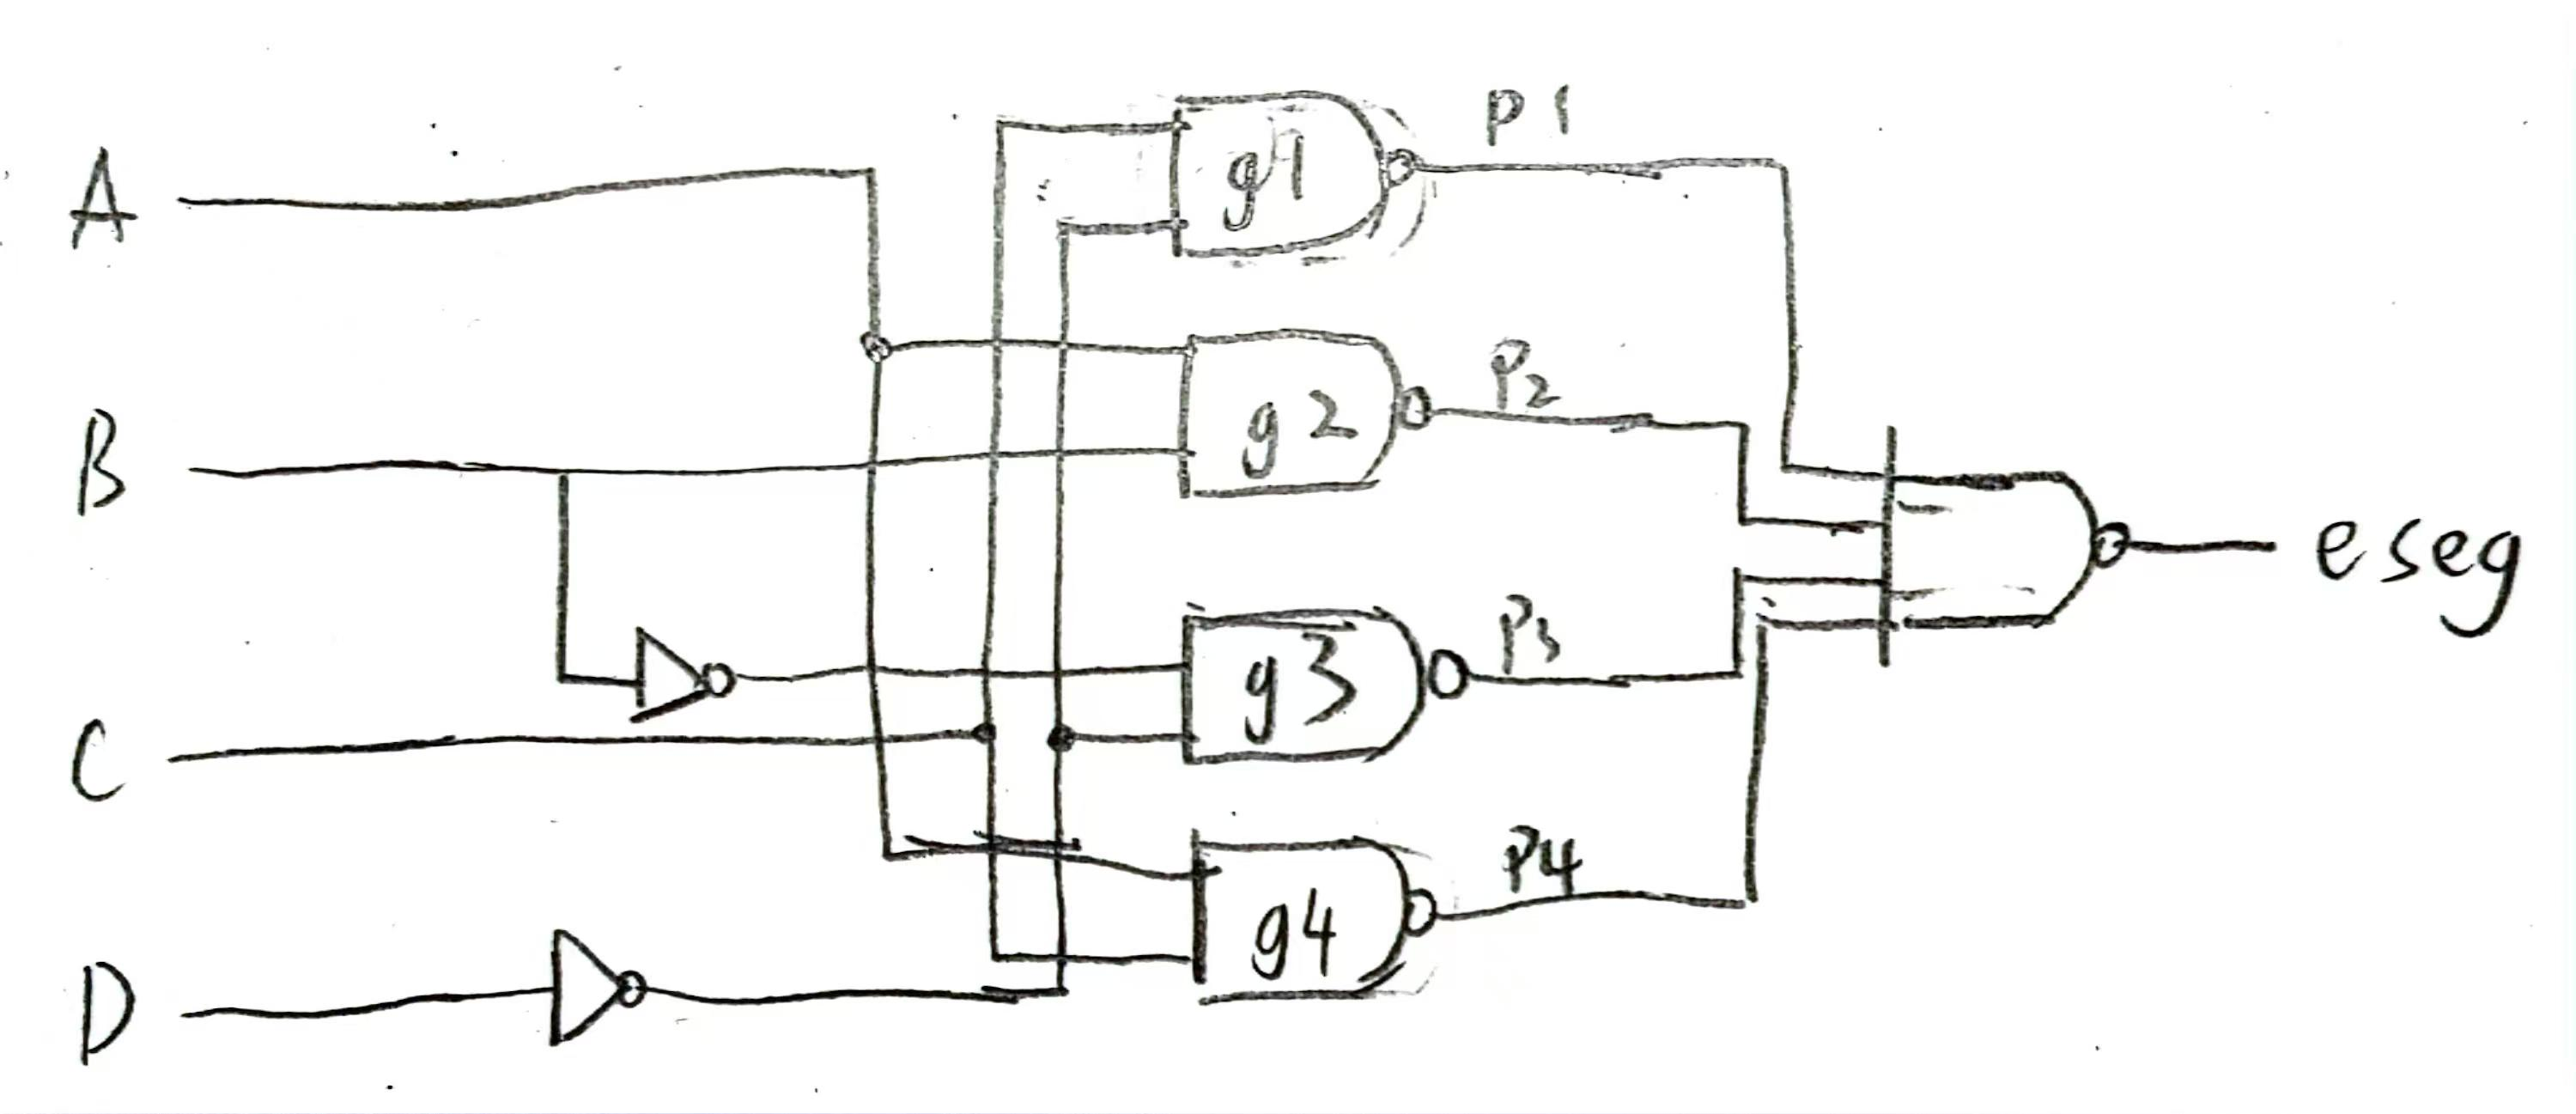
\includegraphics[width=1\textwidth]{binarytoeseg.jpg}
    \label{3to8decoder}
\end{figure}\par
该电路的逻辑表达式是
\begin{align*}
    Eseg = CD'+ AB + B'D' + AC
\end{align*}
\end{document}      
